%%%%%%%%%%%%%%%%%%%%%%%%%%%%%%%%%%%%%%%%%%%%%%%%%%%%
%%% State of the Art
%%%%%%%%%%%%%%%%%%%%%%%%%%%%%%%%%%%%%%%%%%%%%%%%%%%%

\section{State of the Art}
\begin{frame}[noframenumbering]
	\begin{center}
	    \textbf{\huge{State of the Art}}
	\end{center}
\end{frame}

%%% Regime Switching %%%%%
\begin{frame}{Regime Switching}
\begin{figure}[h!]
    \centering
    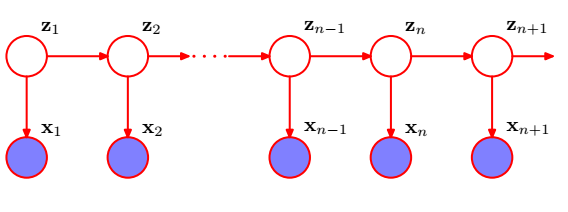
\includegraphics[width=0.5\textwidth]{Figures/hmm1.png}
    %\captionsetup{width=1\linewidth}
    \caption{ Sequential data can be represented by using a Markov chain of latent variables, with each observation conditioned on the state of the corresponding latent variable.}
    %\label{}
\end{figure}
\end{frame}


\begin{frame}{Regime Switching}
\begin{figure}[h!]
    \centering
    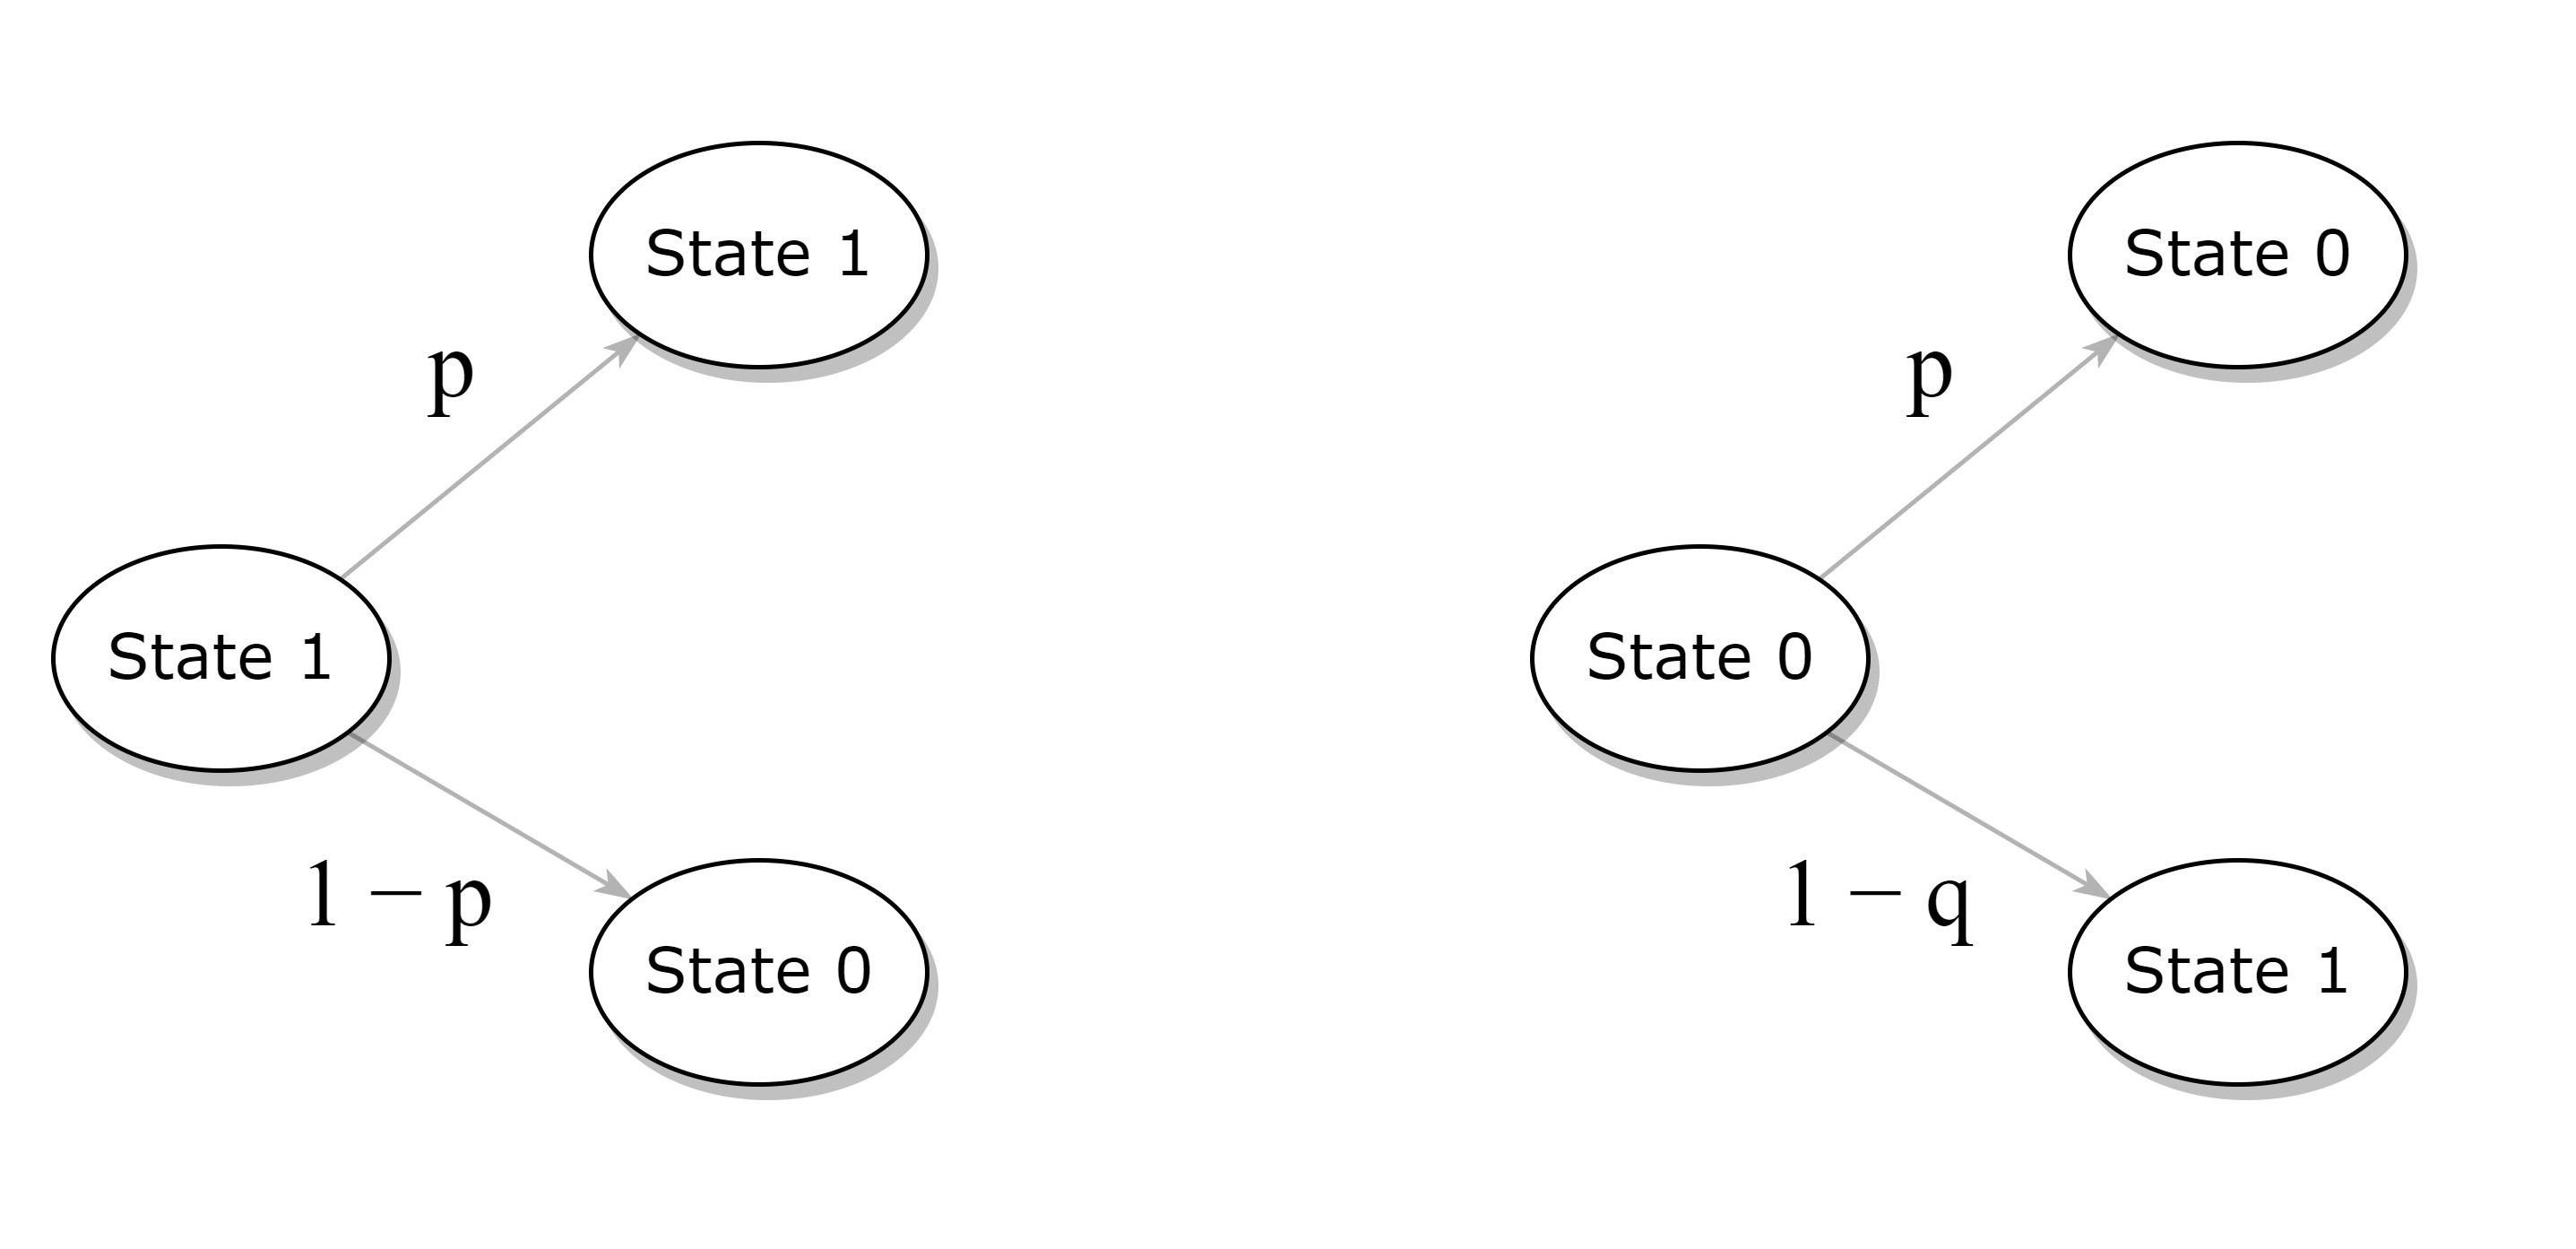
\includegraphics[width=0.7\textwidth]{Figures/markov_chain.jpg}
\end{figure}
\begin{itemize}
    \item The Markov chain depends on 
    \begin{align*}
    A = 
        \begin{pmatrix}
            p & 1-p\\
            1-q & q
        \end{pmatrix}
    \end{align*}
\end{itemize}
\end{frame}


\begin{frame}{Regime Switching - Practical Problems}
 Several problems make Markov models impractical:
\begin{itemize}
    \item \textbf{Optimal number} of states? 
    \item \textbf{Initial conditions} for optimization procedure?
    \item \textbf{frequent rebalancing} can eat up the potential excess return
\end{itemize}
\end{frame}

%%% News Sentiment %%%%%
\begin{frame}{News Sentiment}
News Sentiment in finance:
\begin{itemize}
    \item \cite{tetlock2007giving} is one of the first to show the \textbf{predictive power of News Sentiment}
    \item Further extended to show \textbf{persistence for weeks \& months}\footnote{\citet{uhl2015s}}
    \item \textbf{What about long term usage?}
\end{itemize}
\end{frame}


\begin{frame}{News Sentiment - SAA}
\begin{itemize}
    \item \citet{enhPortOpti} attempt to use \textbf{long-term news sentiment} in an SAA framework
    \item  Black-Litterman (BL) framework + mean variance optimization
    \item \textbf{enhanced} the Sharpe Ratios of the benchmark SAAs by almost 20\%
\end{itemize}
\end{frame}


\begin{frame}{News Sentiment - SAA}
\textbf{Problems with BL \& mean variance}
\begin{itemize}
    \item \textbf{dimensionality curse} of both BL and mean variance
    \item linear views on the assets which are \textbf{assumed to be uncorrelated}
    \item \textbf{hard to quantify} this correlation between views
\end{itemize}
\end{frame}

\begin{frame}{Hierarchical Clustering-Based Asset Allocation}
\textbf{Problem with Markowitz’s approach: }
    \begin{itemize}
            \item Conditioning number of a matrix
            \item \textbf{The more correlated the investments}, the higher the conditioning number
            \item Unstable matrix inversion
     \end{itemize}
\textbf{Markowitz’s curse} states that the more correlated the investments, the greater the need for diversification, and yet the more likely we will receive unstable solutions
   
\end{frame}


\begin{frame}{Hierarchical Clustering-Based Asset Allocation}

\citet{de2016building}:  "Hierarchical clustering refers to the formation of a recursive clustering, suggested by the data, not defined apriori."

    
    \begin{figure}
    \centering
    \begin{minipage}{.5\textwidth}
      \centering
      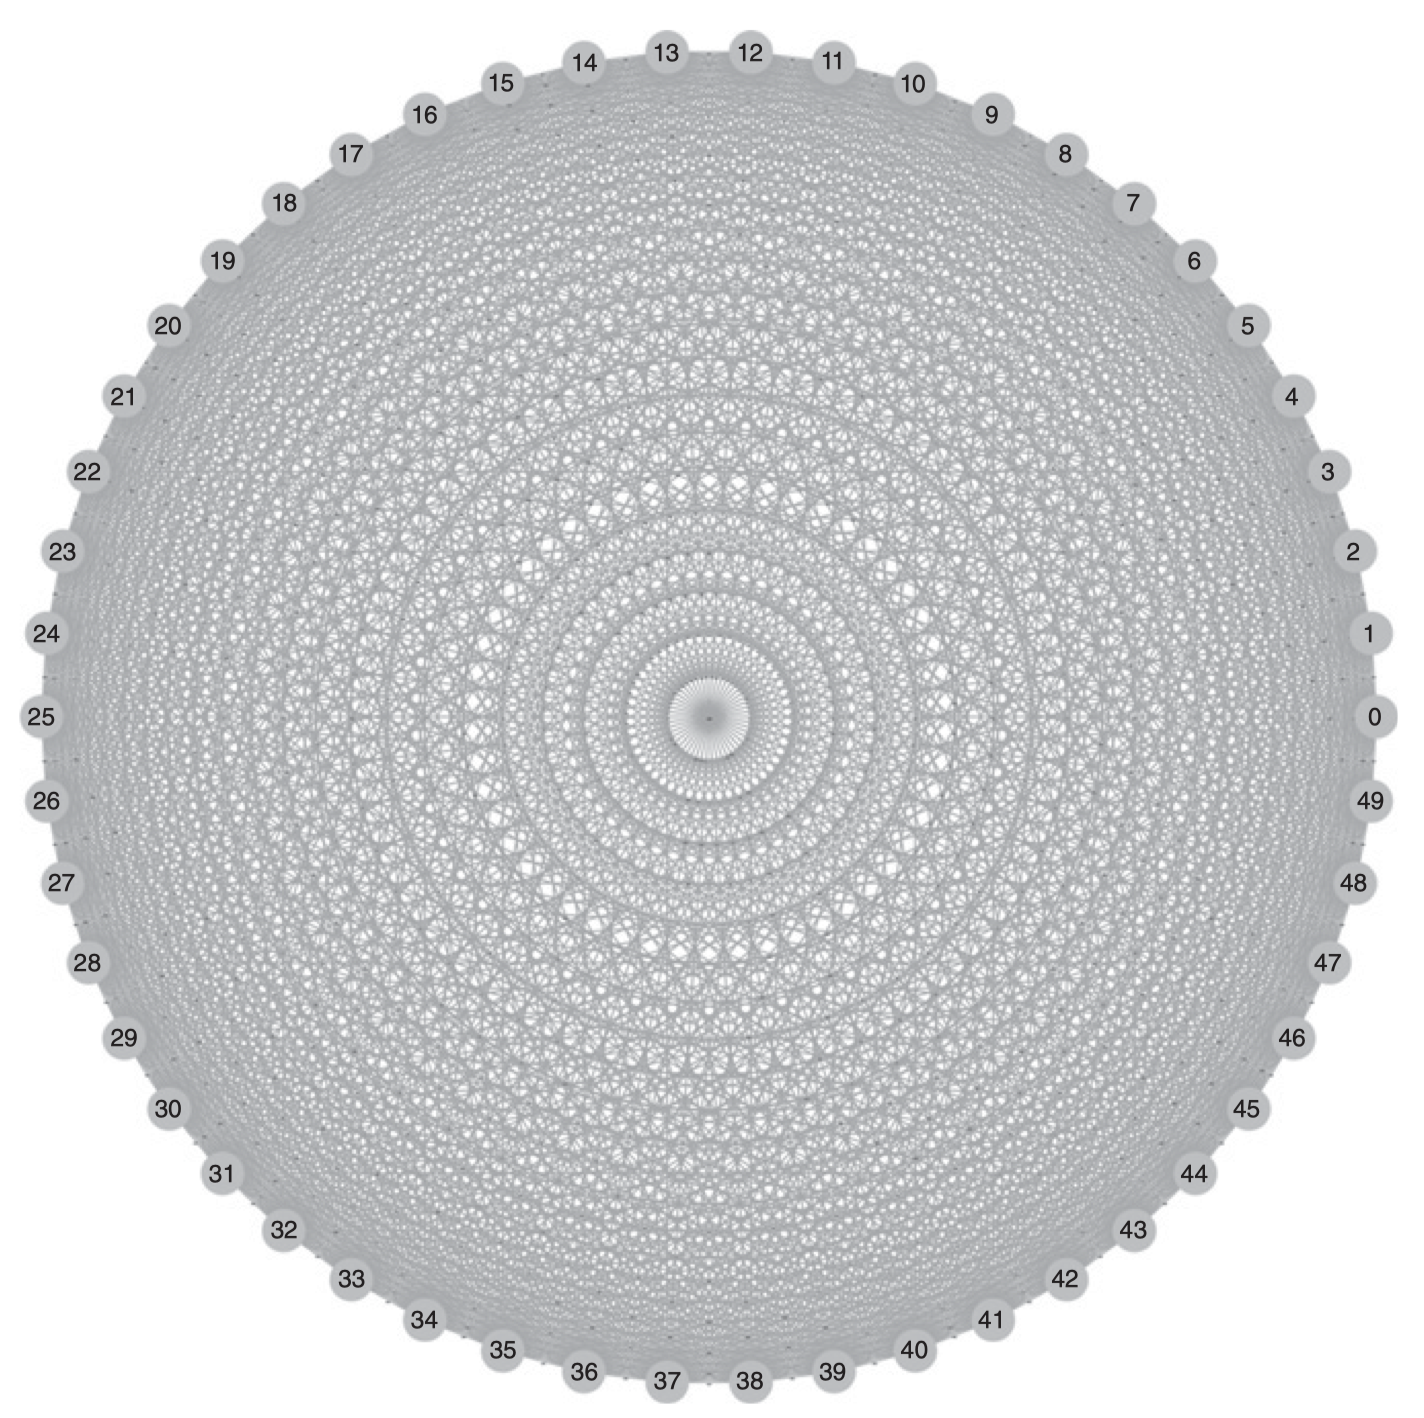
\includegraphics[width=.9\linewidth]{Figures/fuul_matrix.png}
    \end{minipage}%
    \begin{minipage}{.5\textwidth}
      \centering
      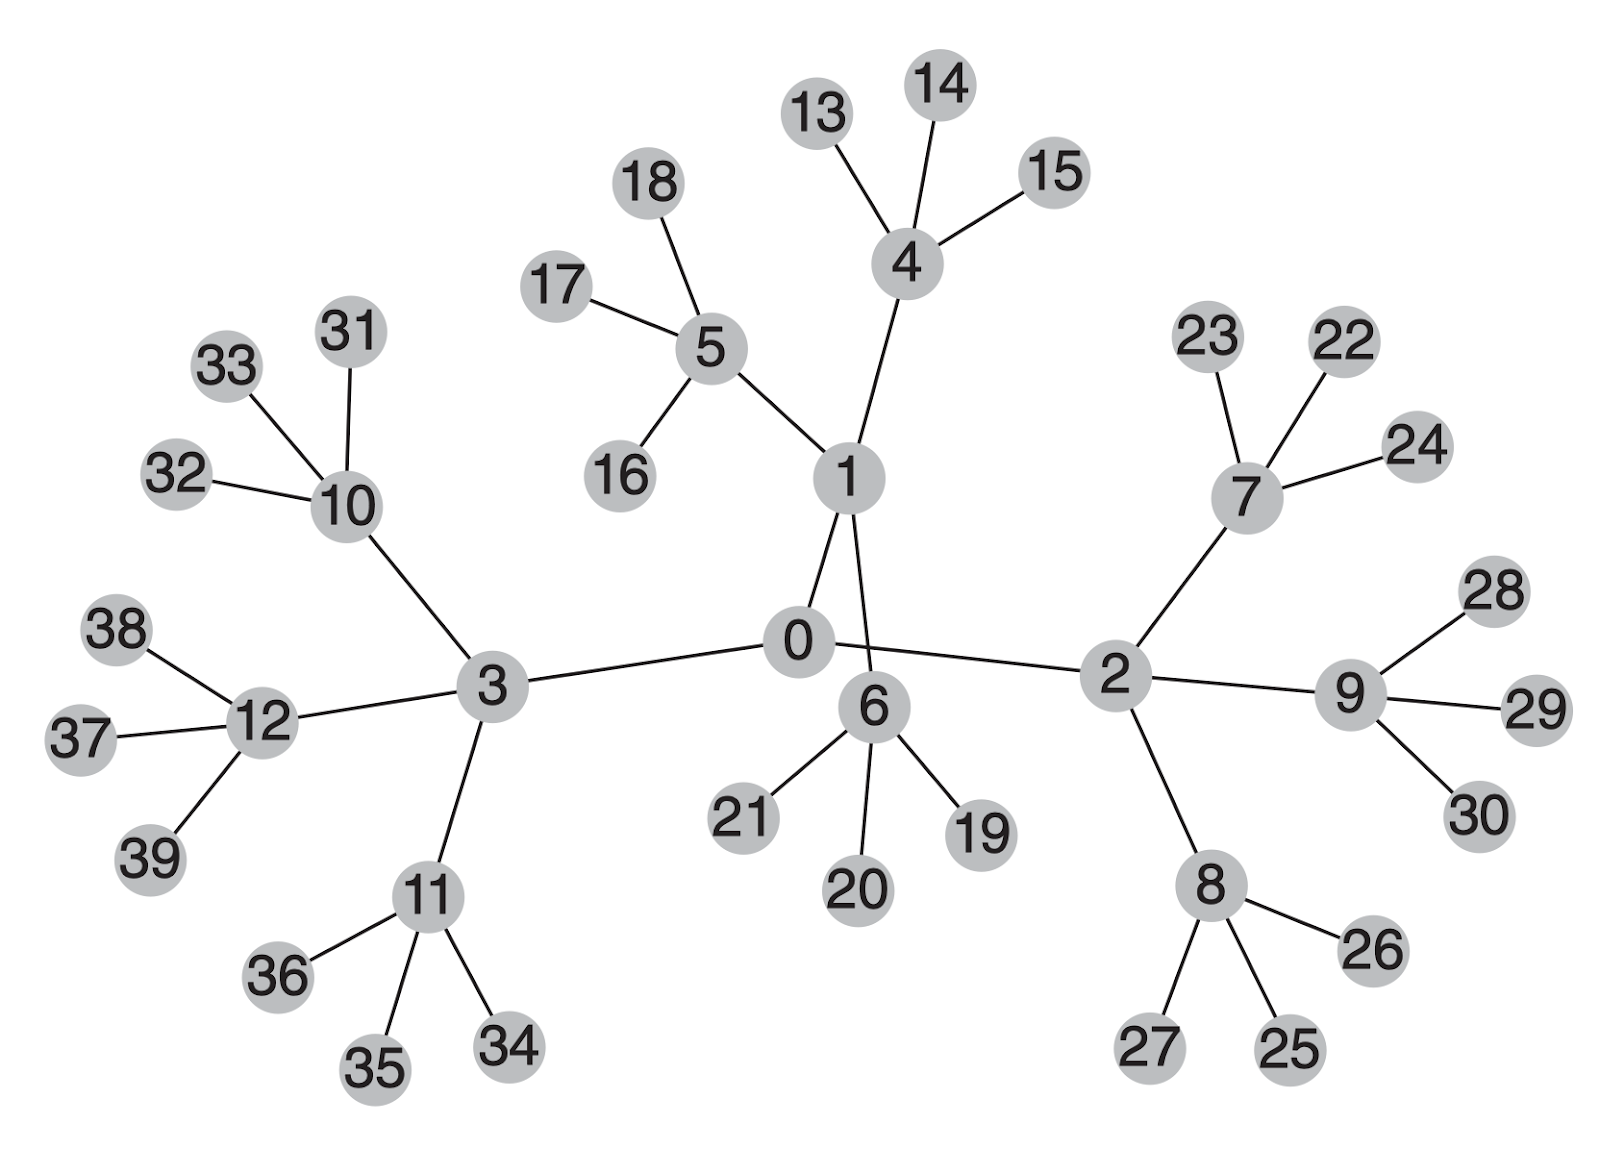
\includegraphics[width=.9\linewidth]{Figures/graph.png}
    \end{minipage}
    \end{figure}
\end{frame}


\begin{frame}{Hierarchical Clustering-Based Asset Allocation}
\textbf{Goal: Construct a binary tree that merges similar clusters.}
    \begin{itemize}
        \item \citet{raffinot2017hierarchical} analyzes four agglomerative clustering algorithms
        \item At each of the $N-1$ steps the closest two (least dissimilar) clusters are merged into a single cluster, producing one less cluster at the next higher level
    \end{itemize}

\end{frame}

\begin{frame}{Hierarchical Clustering-Based Asset Allocation}
    
         Need of a suitable \textbf{distance measure}:
        \begin{align*}
            D_{i,j}=\sqrt{2(1-\rho_{i,j})}
        \end{align*}
        Need a \textbf{measure of dissimilarity} between two clusters $C_i,C_j$:
        \begin{enumerate}
            \item Single Linkage
            \item Complete Linkage
            \item Average Linkage
            \item Ward’s Method
        \end{enumerate}
   

\end{frame}


\begin{frame}{Hierarchical Clustering-Based Asset Allocation - Single}
\textbf{The distance between two clusters is the minimum of the distance between any two points in the clusters.}
    \begin{itemize}
        \item $d_{C_i,C_j}=\min_{x,y}\{D(x,y): x\in C_i, y\in C_j\}$
        \item the most simple one
        \item sensitive to outliers
        \item problem called chaining whereby clusters end up being long and straggly
    \end{itemize}
\end{frame}

\begin{frame}{Hierarchical Clustering-Based Asset Allocation - Complete}
\textbf{The distance between two clusters is the maximum of the distance between any two points in the clusters. }
    \begin{itemize}
        \item $d_{C_i,C_j}=\max_{x,y}\{D(x,y): x\in C_i, y\in C_j\}$
        \item compact clusters of similar size
        \item quite sensitive to outliers
    \end{itemize}
\end{frame}

\begin{frame}{Hierarchical Clustering-Based Asset Allocation - Average}
\textbf{ The distance between two clusters is the average of the distance between any two points in the clusters. }
    \begin{itemize}
        \item $d_{C_i,C_j}=\text{mean}_{x,y}\{D(x,y): x\in C_i, y\in C_j\}$
        \item fairly robust
    \end{itemize}
\end{frame}

\begin{frame}{Hierarchical Clustering-Based Asset Allocation - Ward}
\textbf{The distance between two clusters is the increase of the squared error that results when two clusters are merged.}
    \begin{itemize}
        \item $d_{C_i,C_j}=\frac{m_i m_j}{m_i+m_j}||c_i-c_j||^2$
        \item $m_i,m_j$ are the sizes of the two clusters
        \item $c_i,c_j$ are the centroids for the clusters
        \item  biased towards globular clusters
        \item  less susceptible to noise and outliers
        
    \end{itemize}
\end{frame}